\documentclass[
      aspectratio=169,
        12pt,
    ]{beamer}

% ------------------------------------ font
\usefonttheme[onlymath]{serif}
\usepackage[T1]{fontenc}
\usepackage{textcomp}
\usepackage[scale = 1.0]{tgheros} %Sans serif
\usepackage[scaled]{beramono}
\usepackage{luatexja-otf}
\usepackage[match, deluxe, expert, noto-otf]{luatexja-preset}
\renewcommand{\kanjifamilydefault}{\gtdefault}

% ------------------------------------ math packages
\usepackage{amsmath,amssymb}
\usepackage{siunitx}

% ------------------------------------ comment out package
\usepackage{comment}

% ------------------------------------ tables
\usepackage{longtable, booktabs, array}
\usepackage{threeparttable, threeparttablex, multirow}
\newcolumntype{d}{S[input-symbols = ()]}

% ------------------------------------ figures
\usepackage{graphics, graphicx}
\makeatletter
\def\maxwidth{\ifdim\Gin@nat@width>\linewidth\linewidth\else\Gin@nat@width\fi}
\def\maxheight{\ifdim\Gin@nat@height>\textheight\textheight\else\Gin@nat@height\fi}
\makeatother
% Scale images if necessary, so that they will not overflow the page
% margins by default, and it is still possible to overwrite the defaults
% using explicit options in \includegraphics[width, height, ...]{}
\setkeys{Gin}{width=\maxwidth,height=\maxheight,keepaspectratio}

\usepackage{tikz}
\usetikzlibrary{backgrounds}

% ------------------------------------ other packages (header-includes)

% ------------------------------------ Slide Designs
\definecolor{DarkBlue}{rgb}{0.05, 0.15, 0.35} 

\setbeamercolor{item}{fg=DarkBlue}
\setbeamercolor{title}{fg=DarkBlue}
\setbeamercolor{subtitle}{fg=DarkBlue}
\setbeamercolor{frametitle}{fg=DarkBlue}
\setbeamercolor{section title}{fg=white}

\renewcommand{\textbf}[1]{{\color{DarkBlue}\bfseries#1}}

\setbeamerfont{title}{size=\LARGE,series=\bfseries}
\setbeamerfont{subtitle}{size=\small,series=\bfseries}
\setbeamerfont{institute}{size=\footnotesize}
\setbeamerfont{date}{size=\footnotesize}
\setbeamerfont{section title}{size=\LARGE,series=\bfseries}
\setbeamerfont{frametitle}{size=\Large,series=\bfseries}

\setbeamertemplate{navigation symbols}{}
\setbeamertemplate{footline}[frame number]
\setbeamertemplate{itemize item}[circle]
\setbeamertemplate{itemize subitem}[circle]
\setbeamertemplate{itemize subsubitem}[circle]

\setbeamertemplate{frametitle}{%
  \vspace*{0.5em}\usebeamerfont{frametitle}\insertframetitle\par\vskip-6pt\hrulefill\vspace{-0.1em}
}

\setbeamertemplate{title page}{
    \vfill
    \begingroup
        \centering
        % ------------------------
        \begin{beamercolorbox}[sep=8pt,center]{title}
        \usebeamerfont{title}\inserttitle\par%
        \ifx\insertsubtitle\@empty%
        \else%
            \vskip0.25em%
            {\usebeamerfont{subtitle}\usebeamercolor[fg]{subtitle}\insertsubtitle\par}%
        \fi%     
        \end{beamercolorbox}%
        \hrulefill\vskip0.5em\par
        % ------------------------
        \begin{beamercolorbox}[sep=8pt,center]{author}
        \usebeamerfont{author}\insertauthor
        \end{beamercolorbox}
        \vskip-1em
        % ------------------------
        \begin{beamercolorbox}[sep=8pt,center]{institute}
        \usebeamerfont{institute}\insertinstitute
        \end{beamercolorbox}
        % ------------------------
        \begin{beamercolorbox}[sep=8pt,center]{date}
        \usebeamerfont{date}\insertdate
        \end{beamercolorbox}\vskip0.5em
        % ------------------------
        {\usebeamercolor[fg]{titlegraphic}\inserttitlegraphic\par}
    \endgroup
    \vfill
}

\setbeamertemplate{section page}{%
  
  \begingroup
    \centering
    {\color{white} \hrulefill}\vskip1em
    \begin{beamercolorbox}[sep=8pt, center]{section title}
        \usebeamerfont{section title} \thesection. \insertsection
    \end{beamercolorbox}
    {\color{white} \hrulefill}
  \endgroup
}

\addtobeamertemplate{section page}{%
  \begin{tikzpicture}[remember picture, overlay]
    \useasboundingbox (0,0) rectangle(\the\paperwidth,\the\paperheight);
    \fill[color=DarkBlue!80] (current page.south west) rectangle(current page.north east);
  \end{tikzpicture}
}

\AtBeginSection{\frame{\sectionpage}}

\providecommand{\tightlist}{%
  \setlength{\itemsep}{0pt}\setlength{\parskip}{0pt}}

% ------------------------------------ title information
  \title{骨髄バンクナッジ介入実験}
  \subtitle{解析結果途中報告}
  \author{%
        加藤 大貴\inst{1}
    \and
      }

\begin{document}

\frame{\titlepage}


\begin{frame}
\end{frame}

\begin{frame}{フィールド実験の介入}
\protect\hypertarget{ux30d5ux30a3ux30fcux30ebux30c9ux5b9fux9a13ux306eux4ecbux5165}{}
\begin{itemize}
\tightlist
\item
  対象:骨髄バンクドナー確定後に「適合通知」を受け取るドナー候補者(\(N = 11,154\))
\item
  ドナー候補者確定後、骨髄バンクは対象者に幹細胞提供を依頼する「適合通知」および
  それを郵送した旨を伝えるSNSメーセージを送付
\item
  行動科学の知見に基づいたメッセージを適合通知に加える介入を実施E
\end{itemize}
\end{frame}

\begin{frame}{通常の適合通知の内容}
\protect\hypertarget{ux901aux5e38ux306eux9069ux5408ux901aux77e5ux306eux5185ux5bb9}{}
\begin{quote}
この度、あなたと骨髄バンクの登録患者さんのHLA型(白血球の型)が一致し、
ドナー候補者のおひとりに選ばれました。
今後、ご提供に向け詳しい検査や面談を希望されるかをお伺いしたく連絡させていただきました。
同封の資料をよくお読みいただき、コーディネートが可能かどうか検討の上、
この案内が届いてから7日以内に返信用紙ほかをご返送ください。
返送後、コーディネートを進めさせていただく場合は、
担当者よりご相談のお電話を差し上げますのでよろしくお願い申し上げます。
\end{quote}
\end{frame}

\begin{frame}{介入内容}
\protect\hypertarget{ux4ecbux5165ux5185ux5bb9}{}
\begin{enumerate}
[a.]
\tightlist
\item
  確率メッセージ:「1人の登録患者さんとHLA型が一致するドナー登録者は数百〜数万人に1人です。
  ドナー候補者が複数みつかる場合もありますが、多くはないこともご理解頂ければ幸いです。」
\item
  移植患者情報:「骨髄バンクを介して移植ができる患者さんは現在約6割にとどまっています。
  骨髄等を提供するドナーが早く見つかれば、その比率を高めることができます。」
\end{enumerate}
\end{frame}

\begin{frame}{実験群}
\protect\hypertarget{ux5b9fux9a13ux7fa4}{}
\begin{itemize}
\tightlist
\item
  A群(コントロール):通常の適合通知
\item
  B群(トリートメント1):通常の適合通知+確率メッセージ
\item
  C群(トリートメント2):通常の適合通知+移植患者情報
\item
  D群(トリートメント3):通常の適合通知+確率メッセージ+移植患者情報
\end{itemize}
\end{frame}

\begin{frame}{介入スケジュール}
\protect\hypertarget{ux4ecbux5165ux30b9ux30b1ux30b8ux30e5ux30fcux30eb}{}
週・月の固定効果を取り除くために、実験群は月・週でバランスするように週単位で割り当てた

\begin{table}
\centering
\begin{tabular}[t]{ccccccc}
\toprule
\multicolumn{1}{c}{ } & \multicolumn{6}{c}{月/年} \\
\cmidrule(l{3pt}r{3pt}){2-7}
週 & 9/21 & 10/21 & 11/21 & 12/21 & 1/22 & 2/22\\
\midrule
1 & B & C & C & D & B & A\\
2 & D & B & A & A & C & B\\
3 & A & D & B & C & D & C\\
4 & C & A & D & B & A & D\\
\bottomrule
\end{tabular}
\end{table}
\end{frame}

\begin{frame}{フィールド実験概要}
\protect\hypertarget{ux30d5ux30a3ux30fcux30ebux30c9ux5b9fux9a13ux6982ux8981}{}
\begin{table}
\centering
\fontsize{9}{11}\selectfont
\begin{tabular}[t]{lccccc}
\toprule
\multicolumn{1}{c}{ } & \multicolumn{4}{c}{実験群} & \multicolumn{1}{c}{ } \\
\cmidrule(l{3pt}r{3pt}){2-5}
  & A & B & C & D & p-value\\
\midrule
\addlinespace[0.3em]
\multicolumn{6}{l}{\textbf{A. 介入}}\\
\hspace{1em}通常の適合通知 & X & X & X & X & \\
\hspace{1em}確率メッセージ &  & X &  & X & \\
\hspace{1em}移植患者情報 &  &  & X & X & \\
\addlinespace[0.3em]
\multicolumn{6}{l}{\textbf{B. サンプルサイズ}}\\
\hspace{1em}サンプルサイズ & 2559 & 3075 & 2754 & 2766 & \\
\addlinespace[0.3em]
\multicolumn{6}{l}{\textbf{C. 共変量}}\\
\hspace{1em}年齢 & \num{38.38} & \num{38.13} & \num{37.43} & \num{37.99} & \num{0.06}\\
\hspace{1em}過去のコーディネーション回数 & \num{1.61} & \num{1.59} & \num{1.63} & \num{1.56} & \num{0.36}\\
\hspace{1em}1 = 男性 & \num{0.62} & \num{0.63} & \num{0.63} & \num{0.61} & \num{0.40}\\
\bottomrule
\end{tabular}
\end{table}
\end{frame}

\begin{frame}{アウトカム変数}
\protect\hypertarget{ux30a2ux30a6ux30c8ux30abux30e0ux5909ux6570}{}
アウトカム変数は提供に至るまでのプロセスであり、具体的に以下の6つの工程がある。

\begin{itemize}
\tightlist
\item
  Reply: 適合通知に返信したならば1を取る二値変数
\item
  Intention: 提供を希望するという意向を示して返信したならば1を取る二値変数
\item
  CT: 確認検査を実施したならば1を取る二値変数
\item
  Candidate: 第一候補者に選定されたならば1を取る二値変数
\item
  Consent: 最終同意をしたならば1を取る二値変数
\item
  Donation: 採取をしたならば1を取る二値変数
\end{itemize}
\end{frame}

\begin{frame}{返信~確認検査の二群比較の検定}
\protect\hypertarget{ux8fd4ux4fe1ux78baux8a8dux691cux67fbux306eux4e8cux7fa4ux6bd4ux8f03ux306eux691cux5b9a}{}
\begin{center}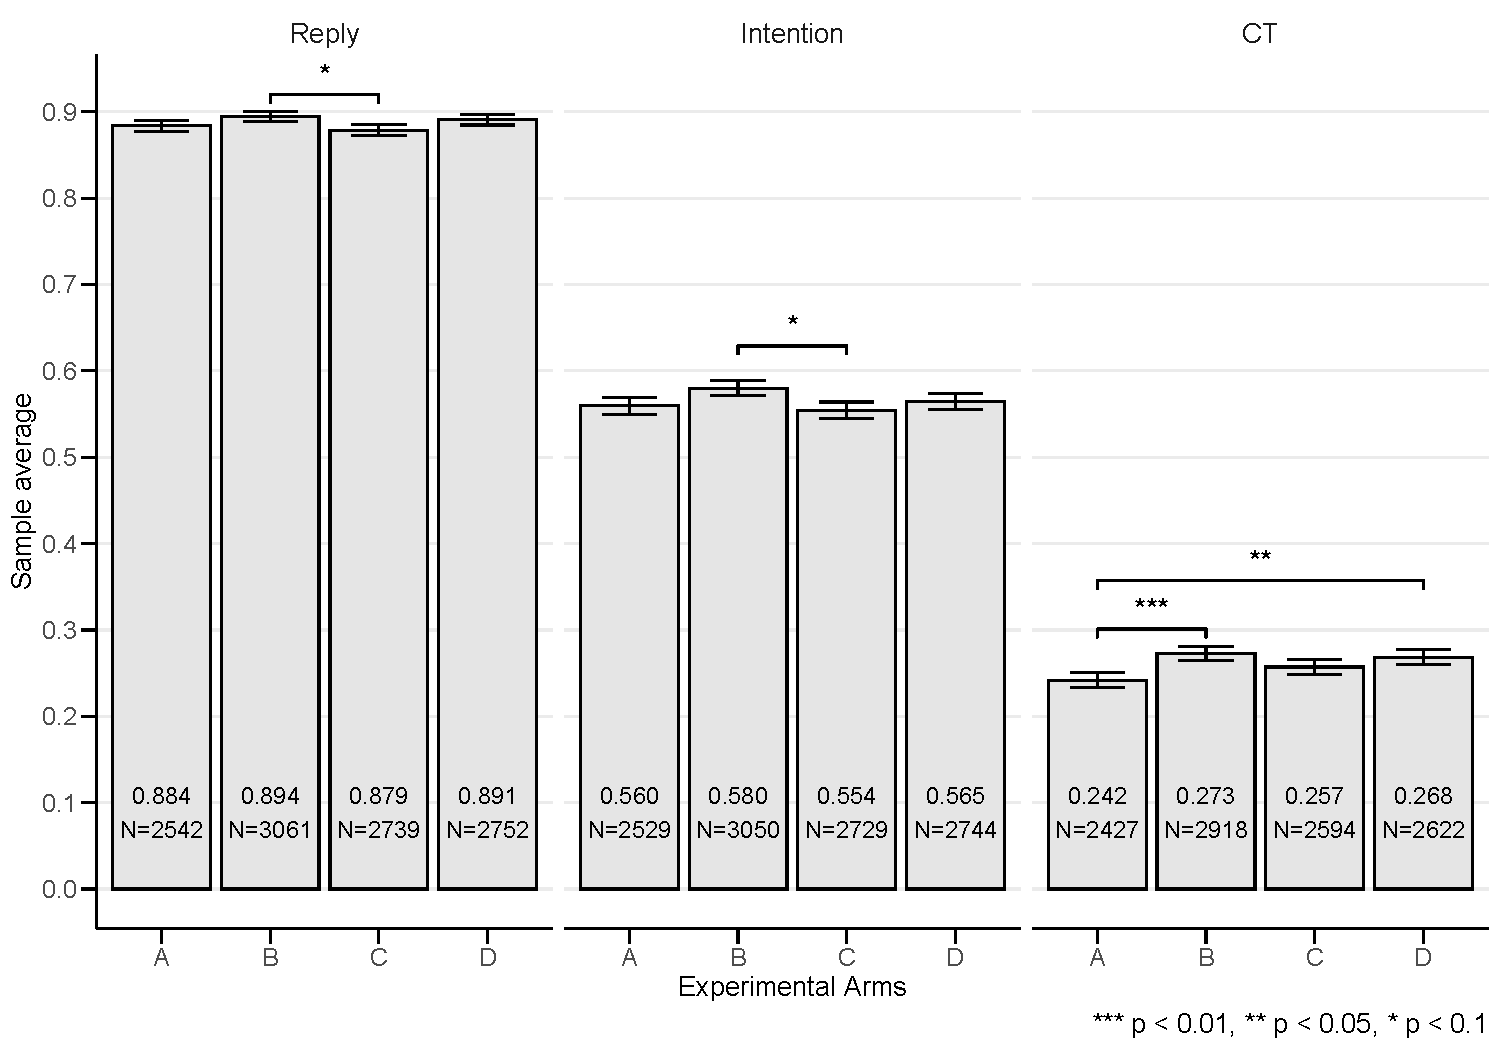
\includegraphics[width=0.75\linewidth]{report_files/figure-beamer/ttest-1-3step-1} \end{center}
\end{frame}

\begin{frame}{候補者選定~採血までの二群比較の検定}
\protect\hypertarget{ux5019ux88dcux8005ux9078ux5b9aux63a1ux8840ux307eux3067ux306eux4e8cux7fa4ux6bd4ux8f03ux306eux691cux5b9a}{}
\begin{center}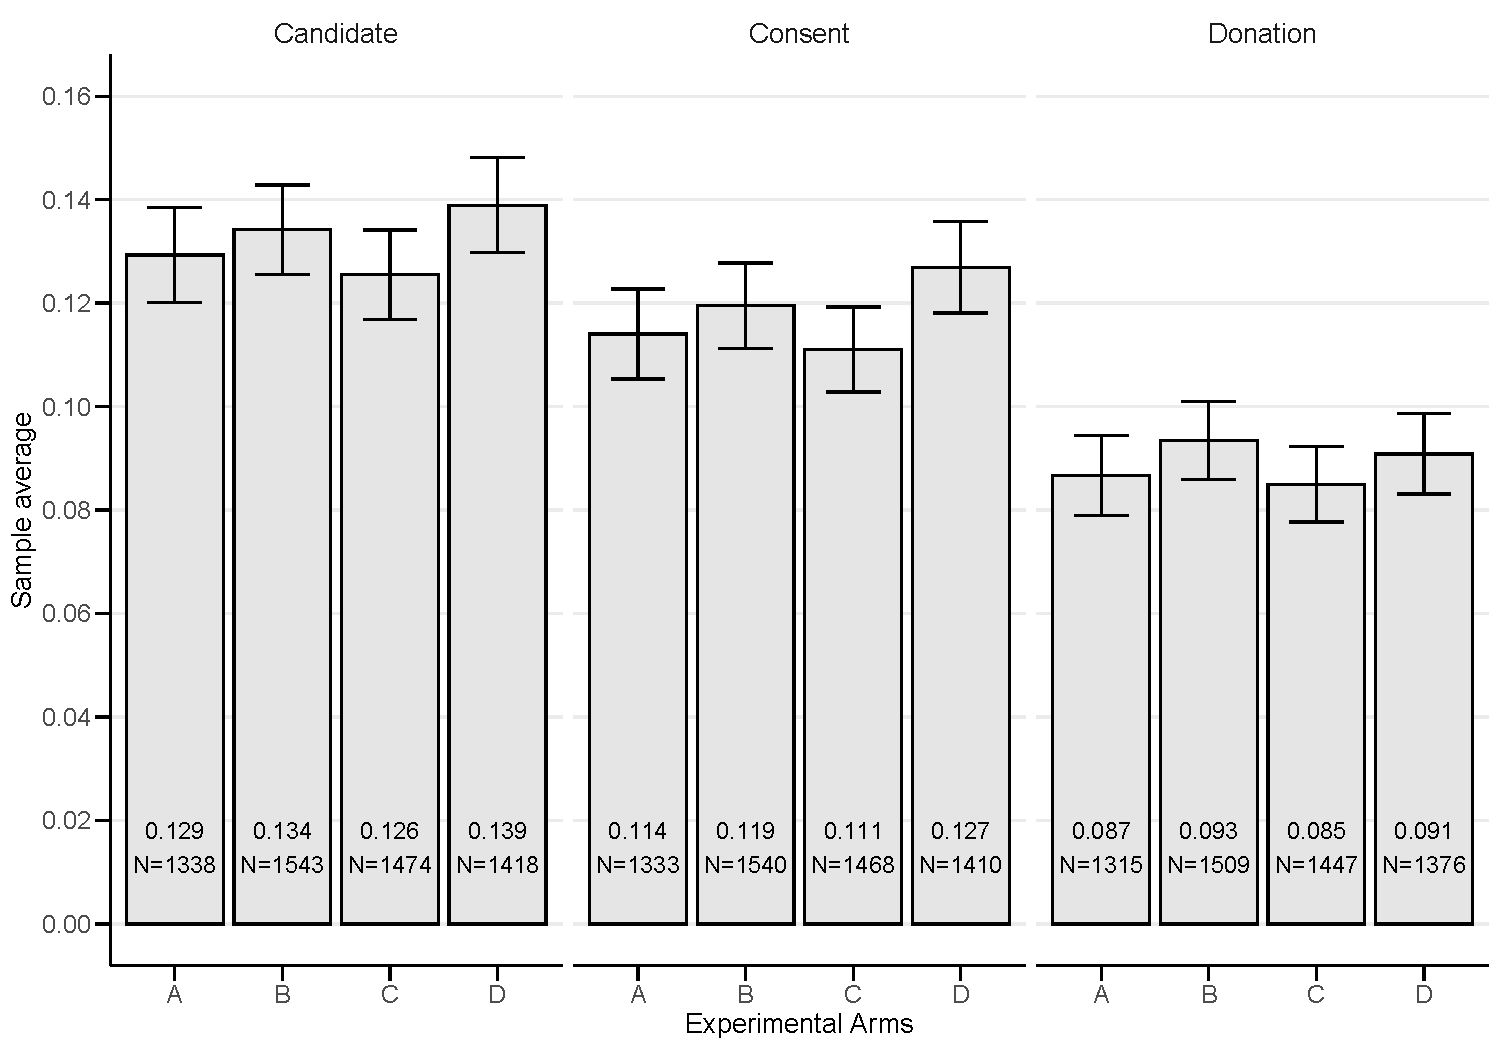
\includegraphics[width=0.75\linewidth]{report_files/figure-beamer/ttest-4-6step-1} \end{center}
\end{frame}

\begin{frame}{線形確率モデル}
\protect\hypertarget{ux7ddaux5f62ux78baux7387ux30e2ux30c7ux30eb}{}
\(m\)月の第\(w\)週に適合通知を受け取った個人\(i\)について、

\[
  Y_{imw} =
  \beta_1 \cdot \text{B}_{mw} + \beta_2 \cdot \text{C}_{mw}
  + \beta_3 \cdot \text{D}_{mw}
  + X'_i \gamma + \lambda_m + \theta_w + u_{imw}
\]

\begin{itemize}
\tightlist
\item
  \(X_i\)は性別・年齢・居住する都道府県・コーディネーション回数
\item
  \(\lambda_m\)と\(\theta_w\)は週・月の固定効果
\end{itemize}
\end{frame}

\begin{frame}{モデル推定結果}
\protect\hypertarget{ux30e2ux30c7ux30ebux63a8ux5b9aux7d50ux679c}{}
\begin{table}
\centering
\fontsize{9}{11}\selectfont
\begin{tabular}[t]{l>{\centering\arraybackslash}p{5em}>{\centering\arraybackslash}p{5em}>{\centering\arraybackslash}p{5em}>{\centering\arraybackslash}p{5em}>{\centering\arraybackslash}p{5em}>{\centering\arraybackslash}p{5em}}
\toprule
  & Reply & Intention & CT & Candidate & Consent & Donation\\
\midrule
B & \num{0.013}** & \num{0.019} & \num{0.034}*** & \num{0.002} & \num{0.002} & \num{0.003}\\
 & (\num{0.006}) & (\num{0.013}) & (\num{0.009}) & (\num{0.009}) & (\num{0.007}) & (\num{0.007})\\
C & \num{0.002} & \num{-0.005} & \num{0.015} & \num{-0.010} & \num{-0.009} & \num{-0.007}\\
 & (\num{0.005}) & (\num{0.011}) & (\num{0.010}) & (\num{0.009}) & (\num{0.007}) & (\num{0.008})\\
D & \num{0.006} & \num{0.006} & \num{0.032}*** & \num{0.008} & \num{0.011} & \num{0.002}\\
 & (\num{0.005}) & (\num{0.010}) & (\num{0.010}) & (\num{0.008}) & (\num{0.007}) & (\num{0.008})\\
\midrule
Num.Obs. & \num{11094} & \num{11052} & \num{10561} & \num{5773} & \num{5751} & \num{5647}\\
\addlinespace[0.3em]
\multicolumn{7}{l}{\textit{F-tests, p-value}}\\
\hspace{1em}B = C & \num{0.015} & \num{0.007} & \num{0.084} & \num{0.293} & \num{0.230} & \num{0.152}\\
\hspace{1em}B = D & \num{0.233} & \num{0.114} & \num{0.857} & \num{0.495} & \num{0.325} & \num{0.917}\\
\hspace{1em}C = D & \num{0.277} & \num{0.164} & \num{0.148} & \num{0.068} & \num{0.018} & \num{0.220}\\
\bottomrule
\multicolumn{7}{l}{\rule{0pt}{1em}* p $<$ 0.1, ** p $<$ 0.05, *** p $<$ 0.01}\\
\end{tabular}
\end{table}
\end{frame}

\begin{frame}{返信スピードに対する効果}
\protect\hypertarget{ux8fd4ux4fe1ux30b9ux30d4ux30fcux30c9ux306bux5bfeux3059ux308bux52b9ux679c}{}
\begin{center}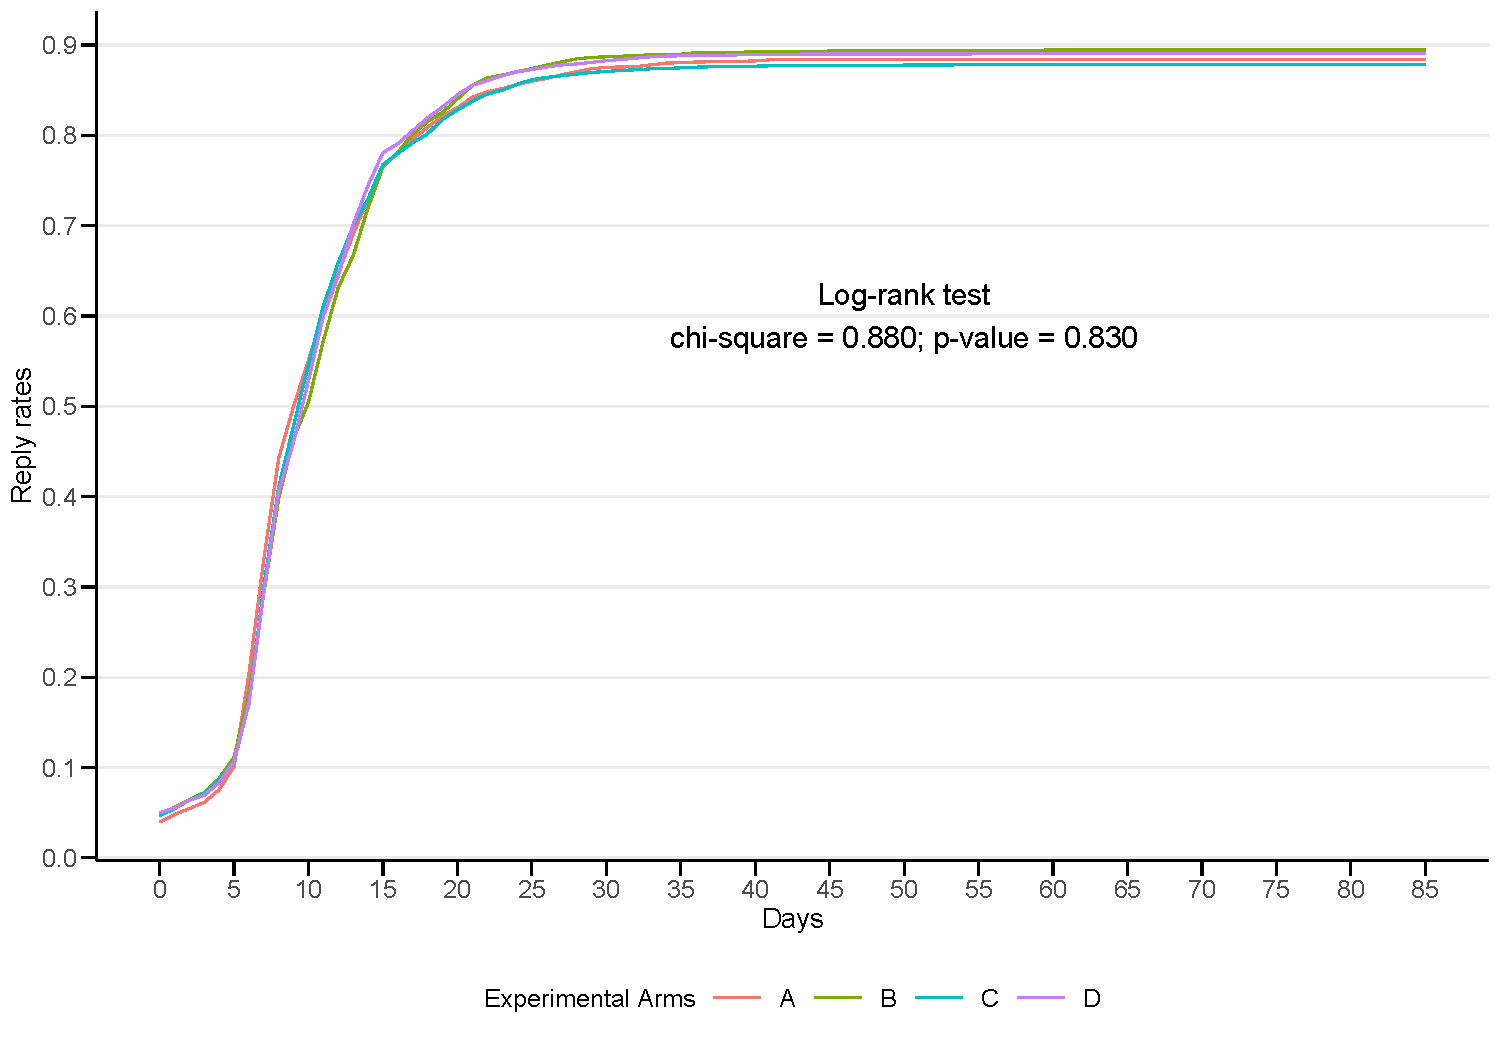
\includegraphics[width=0.75\linewidth]{report_files/figure-beamer/plot-reply-days-1} \end{center}
\end{frame}

\begin{frame}{特定日数までの返信に対する効果}
\protect\hypertarget{ux7279ux5b9aux65e5ux6570ux307eux3067ux306eux8fd4ux4fe1ux306bux5bfeux3059ux308bux52b9ux679c}{}
\begin{table}
\centering
\fontsize{9}{11}\selectfont
\begin{tabular}[t]{l>{\centering\arraybackslash}p{5em}>{\centering\arraybackslash}p{5em}>{\centering\arraybackslash}p{5em}>{\centering\arraybackslash}p{5em}>{\centering\arraybackslash}p{5em}}
\toprule
\multicolumn{1}{c}{ } & \multicolumn{1}{c}{≦ 10days} & \multicolumn{1}{c}{≦ 20days} & \multicolumn{1}{c}{≦ 30days} & \multicolumn{1}{c}{≦ 40days} & \multicolumn{1}{c}{≦ 85days} \\
\cmidrule(l{3pt}r{3pt}){2-2} \cmidrule(l{3pt}r{3pt}){3-3} \cmidrule(l{3pt}r{3pt}){4-4} \cmidrule(l{3pt}r{3pt}){5-5} \cmidrule(l{3pt}r{3pt}){6-6}
  & (1) & (2) & (3) & (4) & (5)\\
\midrule
B & \num{-0.044}*** & \num{0.013} & \num{0.015}** & \num{0.012}* & \num{0.013}**\\
 & (\num{0.014}) & (\num{0.009}) & (\num{0.007}) & (\num{0.006}) & (\num{0.006})\\
C & \num{0.002} & \num{0.007} & \num{0.004} & \num{0.001} & \num{0.002}\\
 & (\num{0.015}) & (\num{0.007}) & (\num{0.006}) & (\num{0.005}) & (\num{0.005})\\
D & \num{-0.028}* & \num{0.018}** & \num{0.007} & \num{0.007} & \num{0.006}\\
 & (\num{0.014}) & (\num{0.007}) & (\num{0.005}) & (\num{0.005}) & (\num{0.005})\\
\midrule
Num.Obs. & \num{11094} & \num{11094} & \num{11094} & \num{11094} & \num{11094}\\
\addlinespace[0.3em]
\multicolumn{6}{l}{\textit{F-tests, p-value}}\\
\hspace{1em}B = C & \num{0.004} & \num{0.282} & \num{0.028} & \num{0.021} & \num{0.015}\\
\hspace{1em}B = D & \num{0.259} & \num{0.474} & \num{0.135} & \num{0.351} & \num{0.233}\\
\hspace{1em}C = D & \num{0.064} & \num{0.022} & \num{0.463} & \num{0.165} & \num{0.277}\\
\bottomrule
\multicolumn{6}{l}{\rule{0pt}{1em}* p $<$ 0.1, ** p $<$ 0.05, *** p $<$ 0.01}\\
\end{tabular}
\end{table}
\end{frame}

\begin{frame}{異質性の検討}
\protect\hypertarget{ux7570ux8ceaux6027ux306eux691cux8a0e}{}
\begin{itemize}
\tightlist
\item
  性別と年齢(30歳以下どうか)でサンプルを分割して、
  各サブサンプル内でメッセージの効果を推定した
\end{itemize}
\end{frame}

\begin{frame}{性別・年齢層別のメッセージBの効果}
\protect\hypertarget{ux6027ux5225ux5e74ux9f62ux5c64ux5225ux306eux30e1ux30c3ux30bbux30fcux30b8bux306eux52b9ux679c}{}
\begin{center}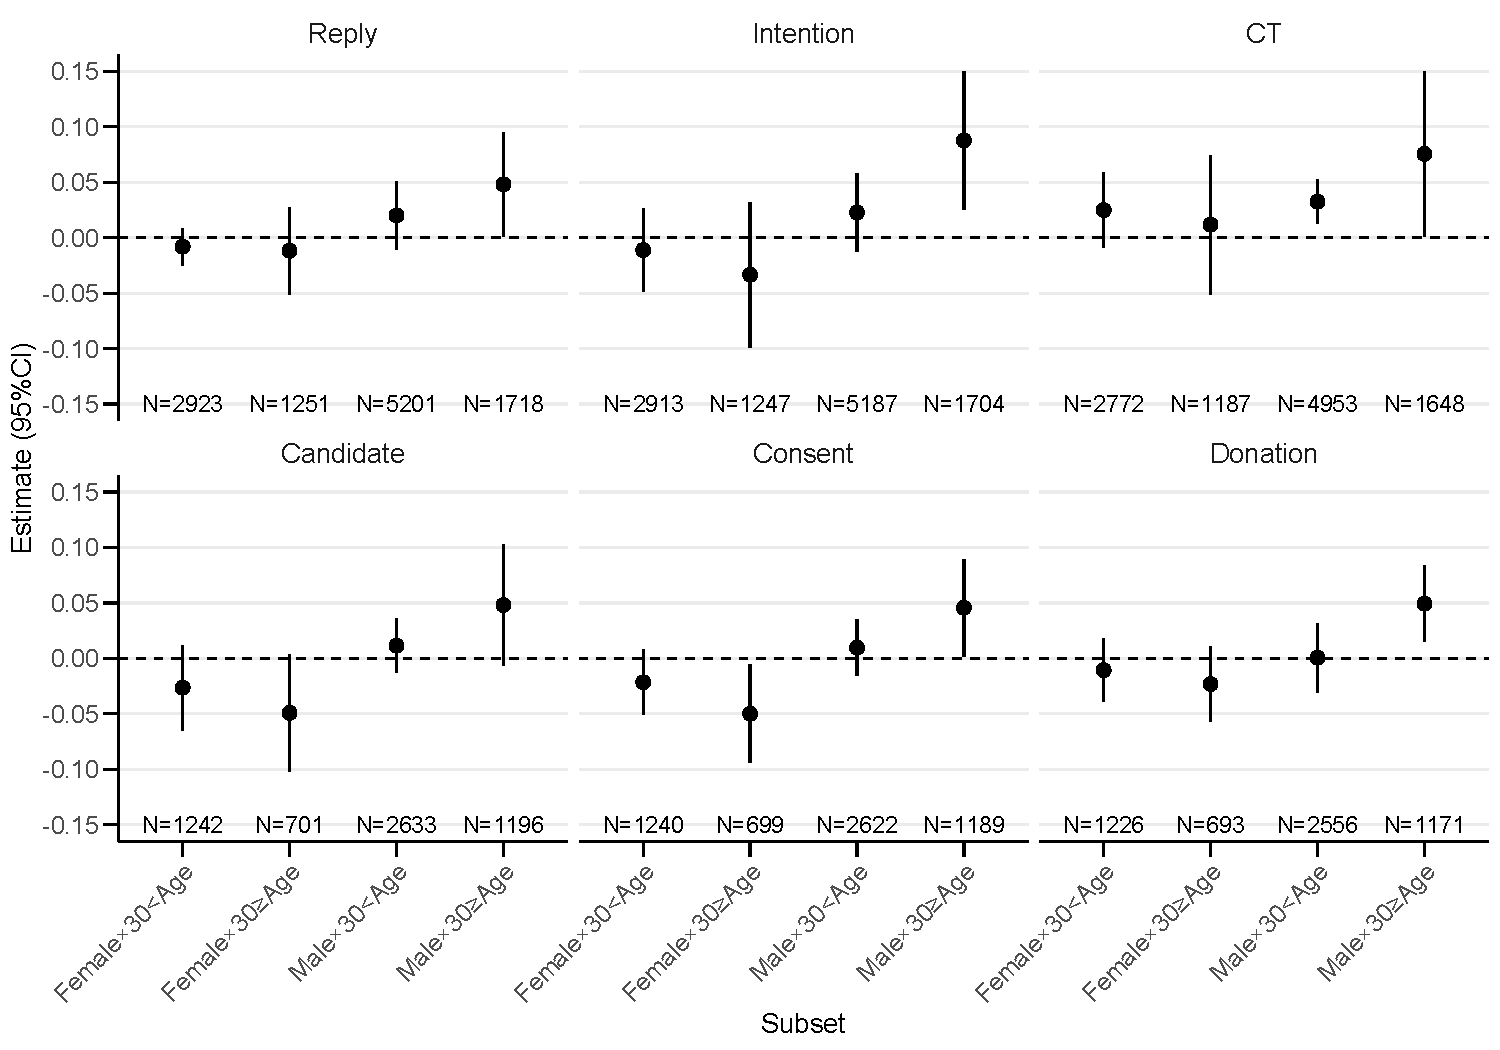
\includegraphics[width=0.75\linewidth]{report_files/figure-beamer/heterogenous-effect-B-1} \end{center}
\end{frame}

\begin{frame}{性別・年齢層別のメッセージCの効果}
\protect\hypertarget{ux6027ux5225ux5e74ux9f62ux5c64ux5225ux306eux30e1ux30c3ux30bbux30fcux30b8cux306eux52b9ux679c}{}
\begin{center}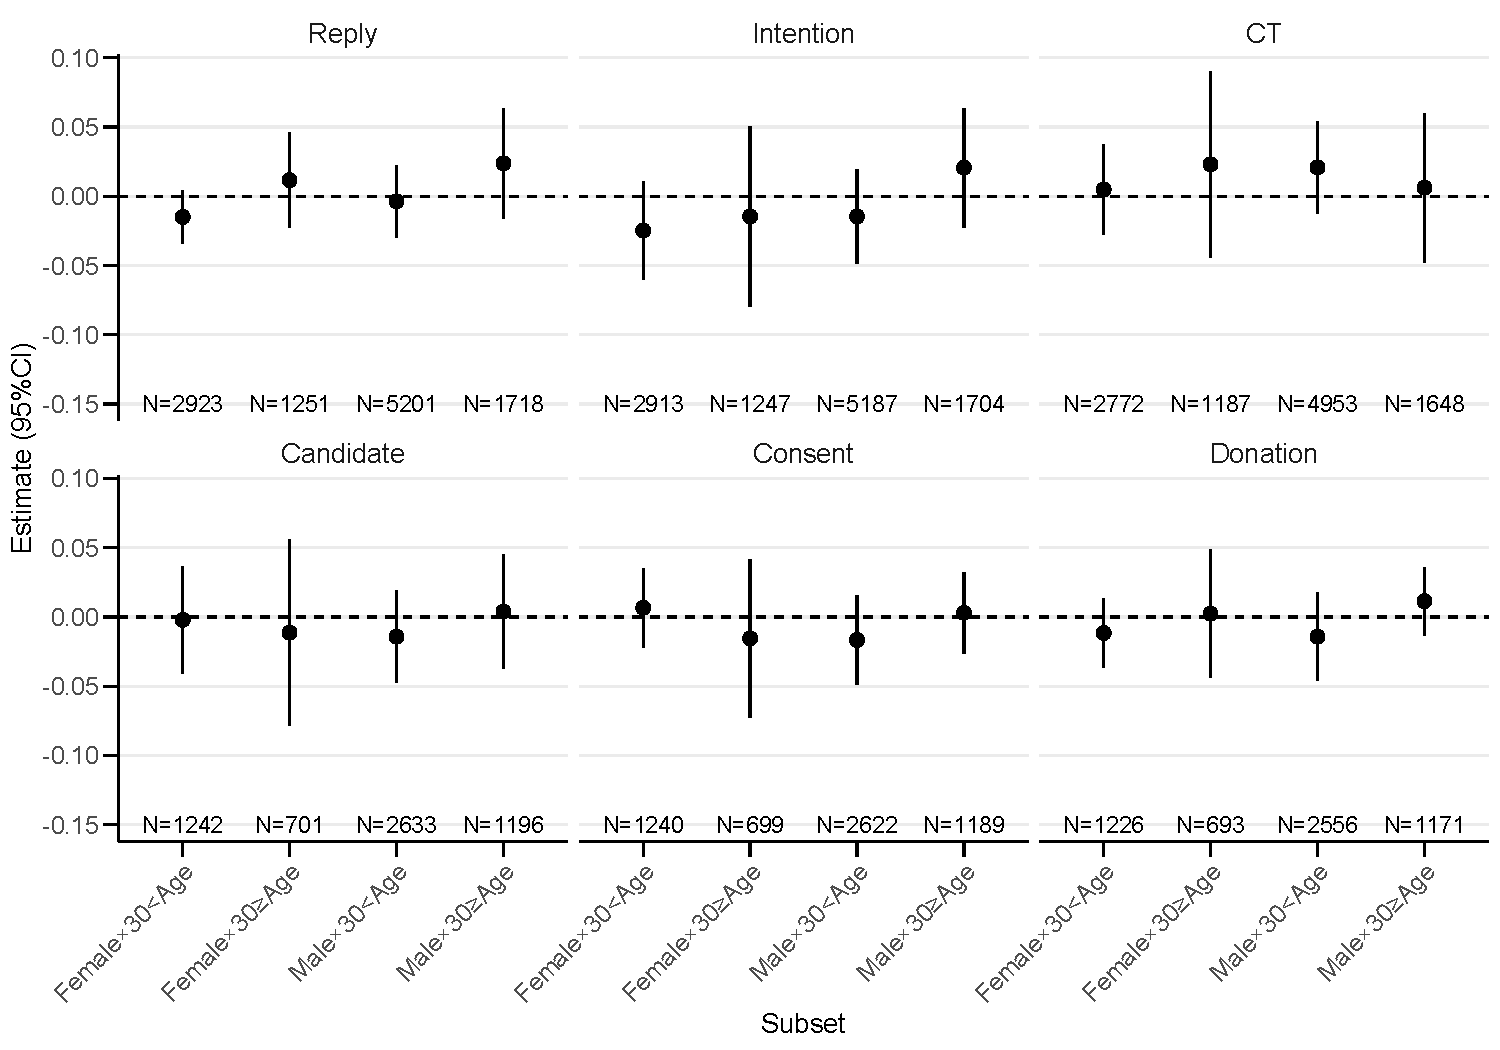
\includegraphics[width=0.75\linewidth]{report_files/figure-beamer/heterogenous-effect-C-1} \end{center}
\end{frame}

\begin{frame}{性別・年齢層別のメッセージDの効果}
\protect\hypertarget{ux6027ux5225ux5e74ux9f62ux5c64ux5225ux306eux30e1ux30c3ux30bbux30fcux30b8dux306eux52b9ux679c}{}
\begin{center}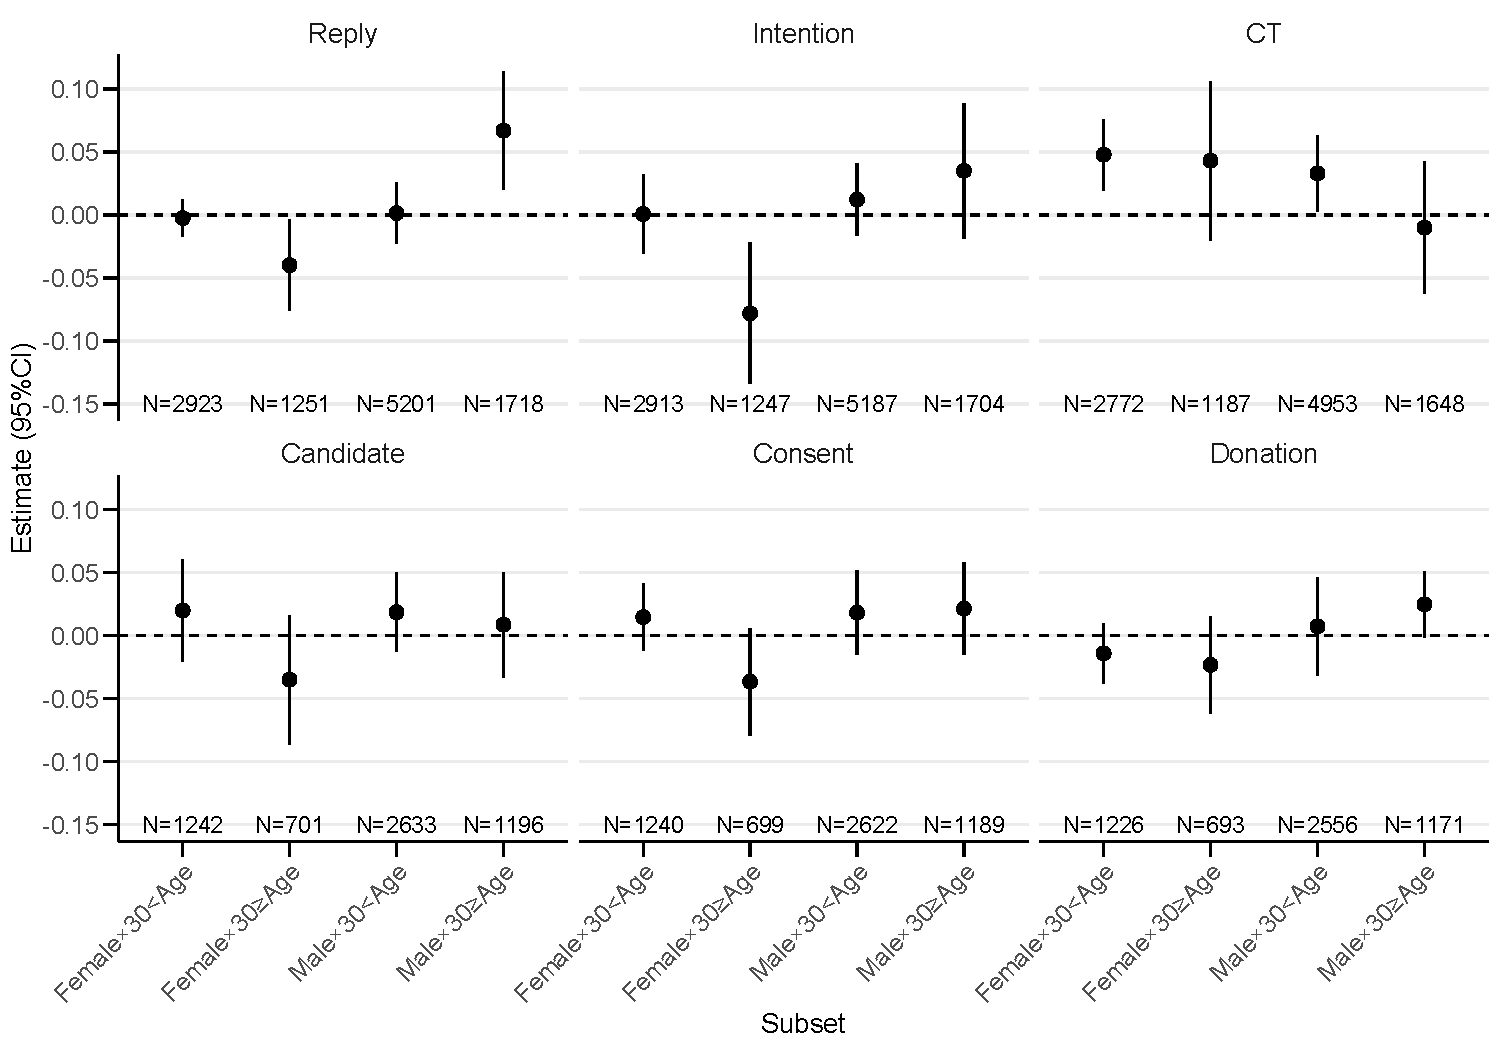
\includegraphics[width=0.75\linewidth]{report_files/figure-beamer/heterogenous-effect-D-1} \end{center}
\end{frame}

\begin{frame}{返信スピードへの効果(30歳以上の女性)}
\protect\hypertarget{ux8fd4ux4fe1ux30b9ux30d4ux30fcux30c9ux3078ux306eux52b9ux679c30ux6b73ux4ee5ux4e0aux306eux5973ux6027}{}
\begin{center}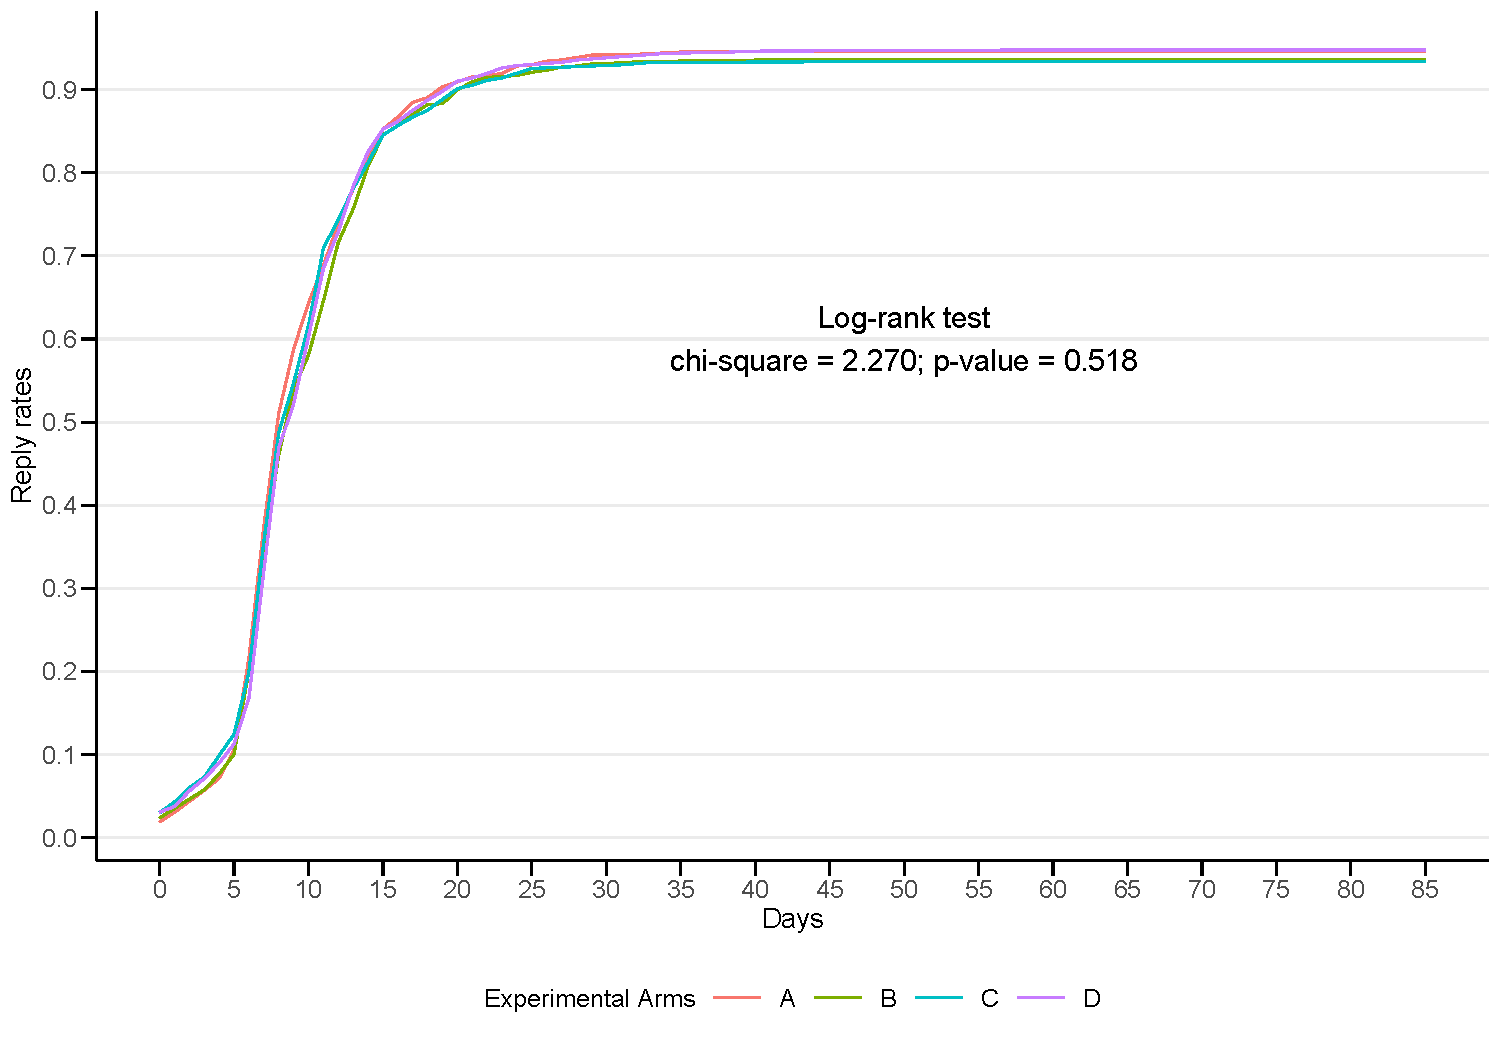
\includegraphics[width=0.75\linewidth]{report_files/figure-beamer/plot-reply-days-female-over30-1} \end{center}
\end{frame}

\begin{frame}{返信スピードへの効果(30歳以下の女性)}
\protect\hypertarget{ux8fd4ux4fe1ux30b9ux30d4ux30fcux30c9ux3078ux306eux52b9ux679c30ux6b73ux4ee5ux4e0bux306eux5973ux6027}{}
\begin{center}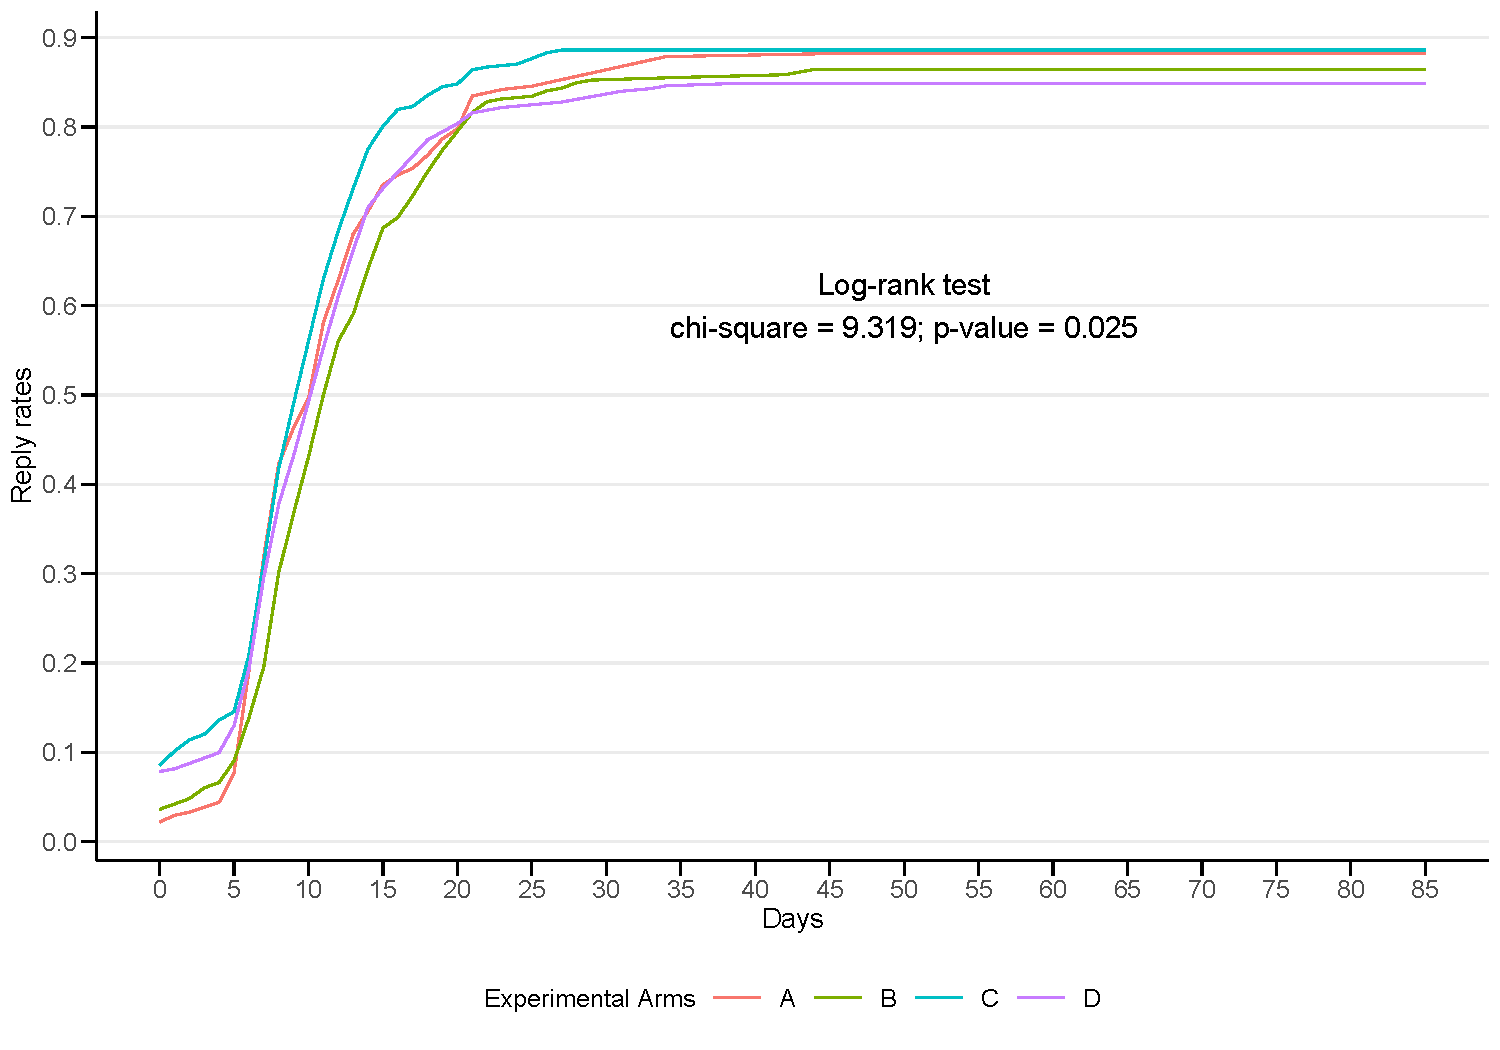
\includegraphics[width=0.75\linewidth]{report_files/figure-beamer/plot-reply-days-female-under30-1} \end{center}
\end{frame}

\begin{frame}{返信スピードへの効果(30歳以上の男性)}
\protect\hypertarget{ux8fd4ux4fe1ux30b9ux30d4ux30fcux30c9ux3078ux306eux52b9ux679c30ux6b73ux4ee5ux4e0aux306eux7537ux6027}{}
\begin{center}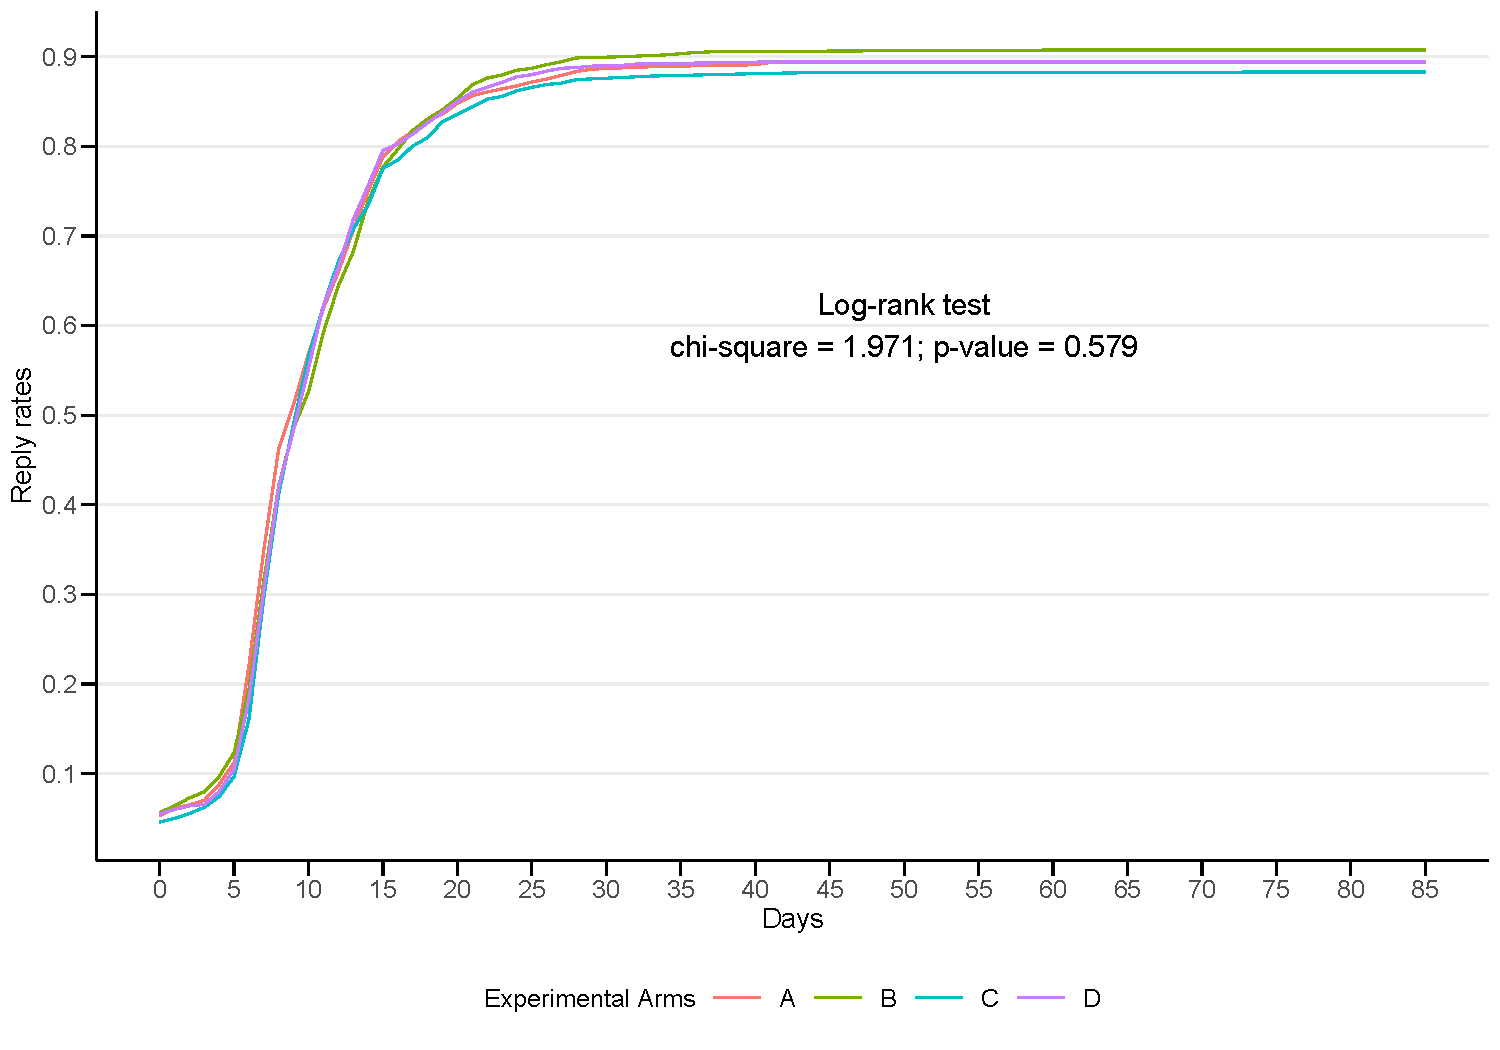
\includegraphics[width=0.75\linewidth]{report_files/figure-beamer/plot-reply-days-male-over30-1} \end{center}
\end{frame}

\begin{frame}{返信スピードへの効果(30歳以下の男性)}
\protect\hypertarget{ux8fd4ux4fe1ux30b9ux30d4ux30fcux30c9ux3078ux306eux52b9ux679c30ux6b73ux4ee5ux4e0bux306eux7537ux6027}{}
\begin{center}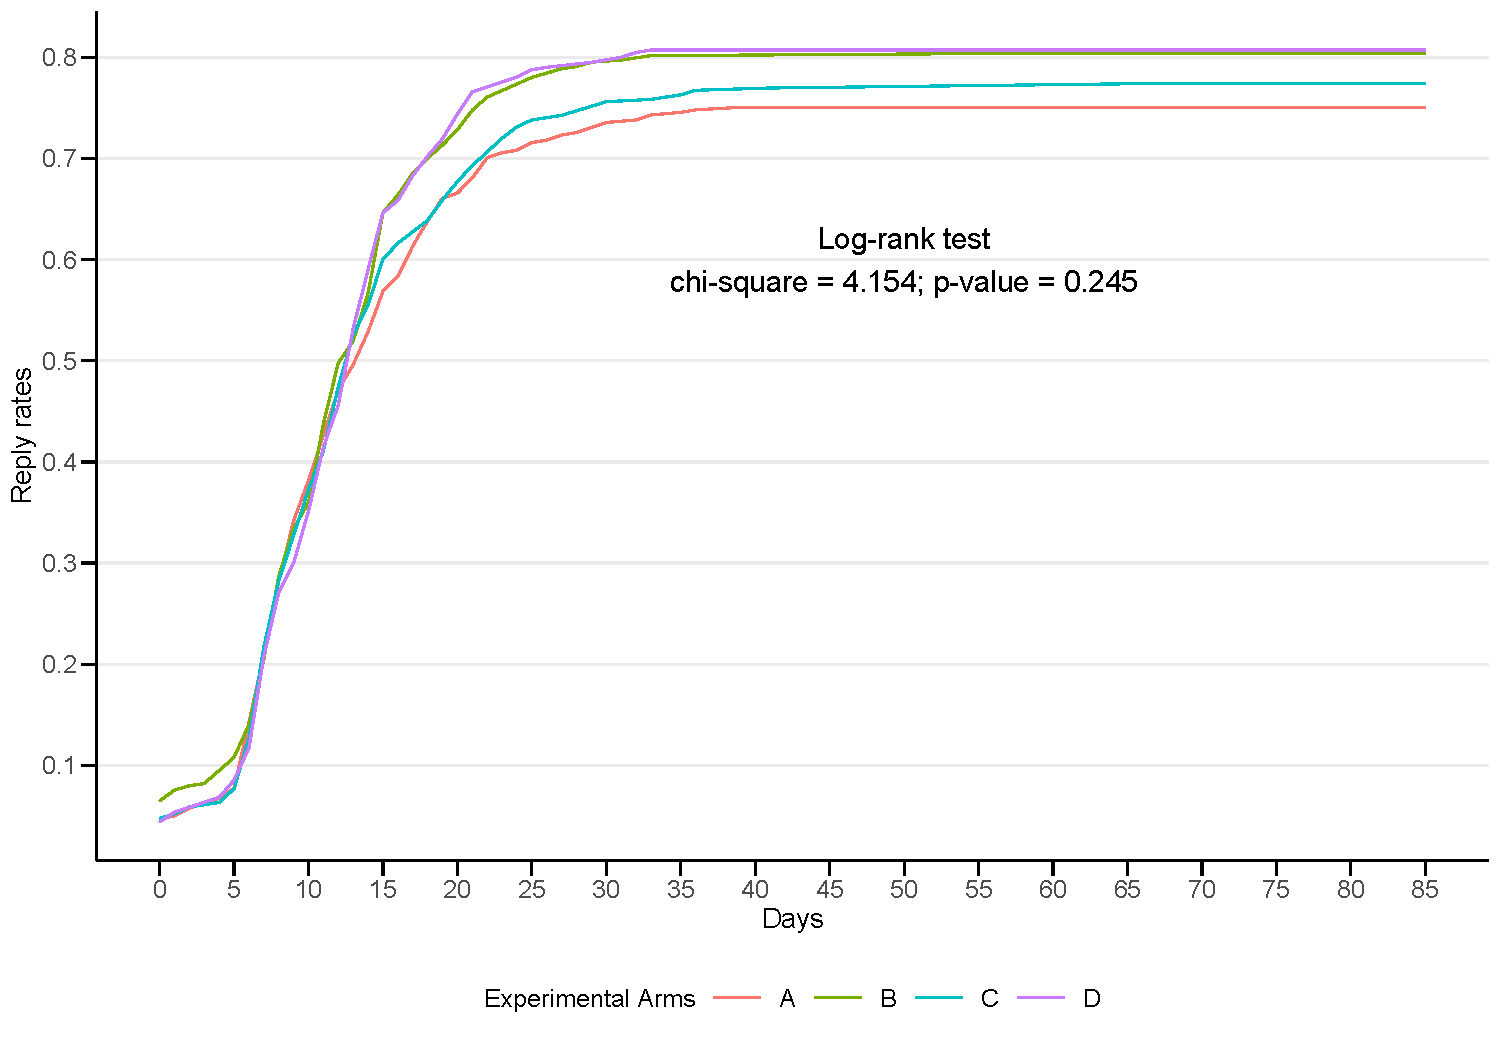
\includegraphics[width=0.75\linewidth]{report_files/figure-beamer/plot-reply-days-male-under30-1} \end{center}
\end{frame}

\begin{frame}{X日以内返信への効果の異質性(30歳以上の女性)}
\protect\hypertarget{xux65e5ux4ee5ux5185ux8fd4ux4fe1ux3078ux306eux52b9ux679cux306eux7570ux8ceaux602730ux6b73ux4ee5ux4e0aux306eux5973ux6027}{}
\begin{table}
\centering
\fontsize{9}{11}\selectfont
\begin{tabular}[t]{l>{\centering\arraybackslash}p{5em}>{\centering\arraybackslash}p{5em}>{\centering\arraybackslash}p{5em}>{\centering\arraybackslash}p{5em}>{\centering\arraybackslash}p{5em}}
\toprule
\multicolumn{1}{c}{ } & \multicolumn{1}{c}{≦ 10days} & \multicolumn{1}{c}{≦ 20days} & \multicolumn{1}{c}{≦ 30days} & \multicolumn{1}{c}{≦ 40days} & \multicolumn{1}{c}{≦ 85days} \\
\cmidrule(l{3pt}r{3pt}){2-2} \cmidrule(l{3pt}r{3pt}){3-3} \cmidrule(l{3pt}r{3pt}){4-4} \cmidrule(l{3pt}r{3pt}){5-5} \cmidrule(l{3pt}r{3pt}){6-6}
  & (1) & (2) & (3) & (4) & (5)\\
\midrule
B & \num{-0.060}* & \num{-0.009} & \num{-0.008} & \num{-0.010} & \num{-0.008}\\
 & (\num{0.030}) & (\num{0.012}) & (\num{0.009}) & (\num{0.008}) & (\num{0.008})\\
C & \num{-0.026} & \num{-0.012} & \num{-0.015} & \num{-0.017}* & \num{-0.015}\\
 & (\num{0.026}) & (\num{0.011}) & (\num{0.010}) & (\num{0.009}) & (\num{0.009})\\
D & \num{-0.048}* & \num{-0.002} & \num{-0.007} & \num{-0.004} & \num{-0.002}\\
 & (\num{0.024}) & (\num{0.009}) & (\num{0.009}) & (\num{0.007}) & (\num{0.007})\\
\midrule
Num.Obs. & \num{2923} & \num{2923} & \num{2923} & \num{2923} & \num{2923}\\
\addlinespace[0.3em]
\multicolumn{6}{l}{\textit{F-tests, p-value}}\\
\hspace{1em}B = C & \num{0.174} & \num{0.704} & \num{0.373} & \num{0.411} & \num{0.415}\\
\hspace{1em}B = D & \num{0.627} & \num{0.201} & \num{0.923} & \num{0.338} & \num{0.345}\\
\hspace{1em}C = D & \num{0.280} & \num{0.122} & \num{0.355} & \num{0.113} & \num{0.122}\\
\bottomrule
\multicolumn{6}{l}{\rule{0pt}{1em}* p $<$ 0.1, ** p $<$ 0.05, *** p $<$ 0.01}\\
\end{tabular}
\end{table}
\end{frame}

\begin{frame}{X日以内返信への効果の異質性(30歳以下の女性)}
\protect\hypertarget{xux65e5ux4ee5ux5185ux8fd4ux4fe1ux3078ux306eux52b9ux679cux306eux7570ux8ceaux602730ux6b73ux4ee5ux4e0bux306eux5973ux6027}{}
\begin{table}
\centering
\fontsize{9}{11}\selectfont
\begin{tabular}[t]{l>{\centering\arraybackslash}p{5em}>{\centering\arraybackslash}p{5em}>{\centering\arraybackslash}p{5em}>{\centering\arraybackslash}p{5em}>{\centering\arraybackslash}p{5em}}
\toprule
\multicolumn{1}{c}{ } & \multicolumn{1}{c}{≦ 10days} & \multicolumn{1}{c}{≦ 20days} & \multicolumn{1}{c}{≦ 30days} & \multicolumn{1}{c}{≦ 40days} & \multicolumn{1}{c}{≦ 85days} \\
\cmidrule(l{3pt}r{3pt}){2-2} \cmidrule(l{3pt}r{3pt}){3-3} \cmidrule(l{3pt}r{3pt}){4-4} \cmidrule(l{3pt}r{3pt}){5-5} \cmidrule(l{3pt}r{3pt}){6-6}
  & (1) & (2) & (3) & (4) & (5)\\
\midrule
B & \num{-0.070}** & \num{0.002} & \num{-0.002} & \num{-0.018} & \num{-0.012}\\
 & (\num{0.028}) & (\num{0.016}) & (\num{0.016}) & (\num{0.019}) & (\num{0.019})\\
C & \num{0.055}** & \num{0.051}*** & \num{0.033}** & \num{0.014} & \num{0.012}\\
 & (\num{0.022}) & (\num{0.016}) & (\num{0.015}) & (\num{0.017}) & (\num{0.017})\\
D & \num{-0.025} & \num{-0.002} & \num{-0.032}** & \num{-0.037}** & \num{-0.040}**\\
 & (\num{0.028}) & (\num{0.012}) & (\num{0.015}) & (\num{0.017}) & (\num{0.017})\\
\midrule
Num.Obs. & \num{1251} & \num{1251} & \num{1251} & \num{1251} & \num{1251}\\
\addlinespace[0.3em]
\multicolumn{6}{l}{\textit{F-tests, p-value}}\\
\hspace{1em}B = C & \num{0.000} & \num{0.000} & \num{0.001} & \num{0.010} & \num{0.035}\\
\hspace{1em}B = D & \num{0.133} & \num{0.646} & \num{0.019} & \num{0.180} & \num{0.058}\\
\hspace{1em}C = D & \num{0.001} & \num{0.000} & \num{0.000} & \num{0.000} & \num{0.000}\\
\bottomrule
\multicolumn{6}{l}{\rule{0pt}{1em}* p $<$ 0.1, ** p $<$ 0.05, *** p $<$ 0.01}\\
\end{tabular}
\end{table}
\end{frame}

\begin{frame}{X日以内返信への効果の異質性(30歳以上の男性)}
\protect\hypertarget{xux65e5ux4ee5ux5185ux8fd4ux4fe1ux3078ux306eux52b9ux679cux306eux7570ux8ceaux602730ux6b73ux4ee5ux4e0aux306eux7537ux6027}{}
\begin{table}
\centering
\fontsize{9}{11}\selectfont
\begin{tabular}[t]{l>{\centering\arraybackslash}p{5em}>{\centering\arraybackslash}p{5em}>{\centering\arraybackslash}p{5em}>{\centering\arraybackslash}p{5em}>{\centering\arraybackslash}p{5em}}
\toprule
\multicolumn{1}{c}{ } & \multicolumn{1}{c}{≦ 10days} & \multicolumn{1}{c}{≦ 20days} & \multicolumn{1}{c}{≦ 30days} & \multicolumn{1}{c}{≦ 40days} & \multicolumn{1}{c}{≦ 85days} \\
\cmidrule(l{3pt}r{3pt}){2-2} \cmidrule(l{3pt}r{3pt}){3-3} \cmidrule(l{3pt}r{3pt}){4-4} \cmidrule(l{3pt}r{3pt}){5-5} \cmidrule(l{3pt}r{3pt}){6-6}
  & (1) & (2) & (3) & (4) & (5)\\
\midrule
B & \num{-0.036}** & \num{0.012} & \num{0.018} & \num{0.021} & \num{0.020}\\
 & (\num{0.017}) & (\num{0.017}) & (\num{0.016}) & (\num{0.016}) & (\num{0.015})\\
C & \num{0.000} & \num{-0.005} & \num{-0.004} & \num{-0.003} & \num{-0.004}\\
 & (\num{0.017}) & (\num{0.013}) & (\num{0.014}) & (\num{0.014}) & (\num{0.013})\\
D & \num{-0.020} & \num{0.005} & \num{0.003} & \num{0.003} & \num{0.002}\\
 & (\num{0.016}) & (\num{0.014}) & (\num{0.013}) & (\num{0.013}) & (\num{0.012})\\
\midrule
Num.Obs. & \num{5201} & \num{5201} & \num{5201} & \num{5201} & \num{5201}\\
\addlinespace[0.3em]
\multicolumn{6}{l}{\textit{F-tests, p-value}}\\
\hspace{1em}B = C & \num{0.055} & \num{0.151} & \num{0.062} & \num{0.046} & \num{0.024}\\
\hspace{1em}B = D & \num{0.397} & \num{0.640} & \num{0.196} & \num{0.131} & \num{0.083}\\
\hspace{1em}C = D & \num{0.310} & \num{0.105} & \num{0.470} & \num{0.464} & \num{0.456}\\
\bottomrule
\multicolumn{6}{l}{\rule{0pt}{1em}* p $<$ 0.1, ** p $<$ 0.05, *** p $<$ 0.01}\\
\end{tabular}
\end{table}
\end{frame}

\begin{frame}{X日以内返信への効果の異質性(30歳以下の男性)}
\protect\hypertarget{xux65e5ux4ee5ux5185ux8fd4ux4fe1ux3078ux306eux52b9ux679cux306eux7570ux8ceaux602730ux6b73ux4ee5ux4e0bux306eux7537ux6027}{}
\begin{table}
\centering
\fontsize{9}{11}\selectfont
\begin{tabular}[t]{l>{\centering\arraybackslash}p{5em}>{\centering\arraybackslash}p{5em}>{\centering\arraybackslash}p{5em}>{\centering\arraybackslash}p{5em}>{\centering\arraybackslash}p{5em}}
\toprule
\multicolumn{1}{c}{ } & \multicolumn{1}{c}{≦ 10days} & \multicolumn{1}{c}{≦ 20days} & \multicolumn{1}{c}{≦ 30days} & \multicolumn{1}{c}{≦ 40days} & \multicolumn{1}{c}{≦ 85days} \\
\cmidrule(l{3pt}r{3pt}){2-2} \cmidrule(l{3pt}r{3pt}){3-3} \cmidrule(l{3pt}r{3pt}){4-4} \cmidrule(l{3pt}r{3pt}){5-5} \cmidrule(l{3pt}r{3pt}){6-6}
  & (1) & (2) & (3) & (4) & (5)\\
\midrule
B & \num{-0.024} & \num{0.073}** & \num{0.058}*** & \num{0.046}* & \num{0.048}**\\
 & (\num{0.036}) & (\num{0.031}) & (\num{0.021}) & (\num{0.023}) & (\num{0.023})\\
C & \num{-0.001} & \num{0.025} & \num{0.024} & \num{0.016} & \num{0.024}\\
 & (\num{0.037}) & (\num{0.027}) & (\num{0.018}) & (\num{0.019}) & (\num{0.019})\\
D & \num{-0.018} & \num{0.105}*** & \num{0.071}*** & \num{0.067}*** & \num{0.067}***\\
 & (\num{0.034}) & (\num{0.026}) & (\num{0.019}) & (\num{0.023}) & (\num{0.023})\\
\midrule
Num.Obs. & \num{1718} & \num{1718} & \num{1718} & \num{1718} & \num{1718}\\
\addlinespace[0.3em]
\multicolumn{6}{l}{\textit{F-tests, p-value}}\\
\hspace{1em}B = C & \num{0.502} & \num{0.114} & \num{0.104} & \num{0.166} & \num{0.255}\\
\hspace{1em}B = D & \num{0.851} & \num{0.302} & \num{0.605} & \num{0.445} & \num{0.490}\\
\hspace{1em}C = D & \num{0.653} & \num{0.002} & \num{0.015} & \num{0.018} & \num{0.045}\\
\bottomrule
\multicolumn{6}{l}{\rule{0pt}{1em}* p $<$ 0.1, ** p $<$ 0.05, *** p $<$ 0.01}\\
\end{tabular}
\end{table}
\end{frame}

\end{document}
